\documentclass[border=10pt]{standalone}
\usepackage{pgfplots}
\usepgfplotslibrary{polar}
\pgfplotsset{compat=1.18, trig format plots=deg}
\begin{document}
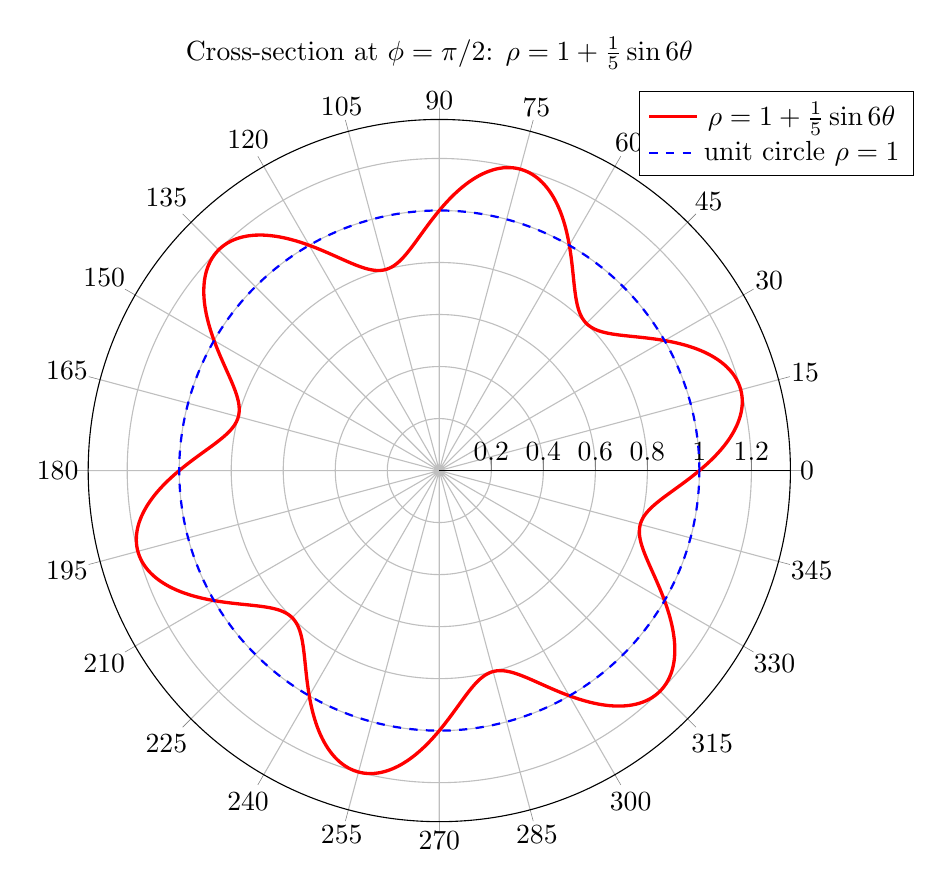
\begin{tikzpicture}
\begin{polaraxis}[
    width=10.5cm, height=10.5cm,
    samples=600, domain=0:360,
    ymax=1.35, ymin=0,
    grid=both,
    ytick={0.2,0.4,0.6,0.8,1.0,1.2},
    title={Cross-section at $\phi=\pi/2$: $\rho = 1+\frac{1}{5}\sin 6\theta$}]
\addplot[red, very thick] {1+0.2*sin(6*x)};
\addlegendentry{$\rho=1+\frac15\sin 6\theta$}
\addplot[blue, thick, dashed] {1};
\addlegendentry{unit circle $\rho=1$}
\end{polaraxis}
\end{tikzpicture}
\end{document}
